Although high accuracy tagging tools are generally available, sometimes their performance is not satisfactory and shall be increased further.
In cases, when very high annotation quality is required, variance of tools should be considered.
Disparate methods can result in different sort of errors, therefore their combination can yield better algorithms.
Even though, this idea is not new, being present in both machine learning and \acrshort{nlp} literature, there have not been much work for morphologically rich languages. 

In this section, the case of agglutinative languages is investigated by experimenting with Hungarian morphological disambiguator tools.
First, we give a brief overview about \acrshort{pos} tagger combination methods.
Next, discrepancies of two taggers are presented allowing us to create a new combination architecture.
Finally, we evaluate the proposed method by measuring its improvement over baseline tools used.

\subsection{Background}

The design process of a combined tagger system involves several steps\footnote{Statements are based on studies of Brill and Wu~\cite{Brill1998} and Halteren et al.~\cite{Halteren2001}.}.
First, it needs to be examined whether the errors of components are different enough to outperform the best individual system significantly.
Then an appropriate combining scheme must be found.
Decisions to be made by a combination algorithm can be of at least two sorts: 
\begin{enumerate}
  \item it can either always select the output of one of the bottom-level systems, or 
  \item it can generate an output of its own that may differ from the output of each individual embedded system. 
\end{enumerate}

When applying the former solution, errors of embedded systems determine a theoretical upper limit on the accuracy of the combined system, since it can never generate the expected output whenever neither of the embedded classifiers generate it.
Thus, the latter solution seems more beneficial in theory.
However, the complexity of the annotation task to be performed and the available training data may have an influence on which of these options is feasible and how they perform in practice.
E.g. if the cardinality of the output annotation and features involved in training is high, there may be either data sparseness or performance problems with the second option.

As regards combination strategies, a basic method is majority voting.
Other, more advanced, schemes involve training a top-level classifier basing on the individual embedded systems.
This class of schemes is commonly referred to as stacking learners.
In doing so, the top-level classifier may use various features of both the inputs and the outputs of the bottom-level classifiers when making its decision. 

One of the first attempts of combining English PoS taggers was presented by Brill and Wu \cite{Brill1998}.
They propose memory-based learning which employs contextual and lexical clues.
In their experiments, the solution where the top-level learner always selects the output of one of the embedded taggers outperformed the more general scheme that allowed the output differ from either of the proposed tags.
Next, a comprehensive study by van Halteren et al. \cite{Halteren2001} details an overview of previous combination attempts.
Further on, the authors show that cross-validation can be used to train top-level classifiers for an optimal utilization of the corpus.
They found a scheme performing best characterized as generalized voting.
Although it can yield annotation differing from the output of the embedded taggers, it can also be interpreted as a stacking method.
However, the cardinality of the tag set and the dimensionality of the feature space was modest compared to that in our case.

A system of different architecture is presented by Hajič et al. \cite{Hajic2001}: in contrast to the parallel and hierarchical architecture of the systems above, it employs a serial combination of annotators starting with a rule-based morphological analyzer, followed by constraint-based filters feeding statistical taggers at the end of the chain. 

We use metalearners with cross-validation, since such schemes \cite{Brill1998,Halteren2001} perform effectively.
Further on language-specific symbolic components are utilized as well, as they can help to handle the rich morphology of the target language.
%In that way, we improve existing methods. 
First, the underlying architecture of general combination methods is modified to produce lemmata candidates as well.
Then, features investigated which fit the best for agglutinative languages.

\subsection{Discrepancies of taggers}

Evaluating taggers on general Hungarian can show that two of the best performing tools (our new method and HuLaPos) significantly diverge by the errors they made.
In doing so, a detailed analysis of errors is carried out first, aiming to reveal their possible combined performance.
For this, we rely on the Humor-tagged Szeged Corpus.
It is split to 3 parts: 80\% of the sentences is utilized for training the systems, 10\% is employed for development purposes while the rest is set apart for final evaluation (cf. Table \ref{comb-data}).

\begin{table}[H]
\centering
\caption{Sentences and tokens of the corpus used}\label{tab:comb-data}
\begin{tabular}{l r r}
\hline
& Tokens & Sentences \\
\hline
Training set & 98,225 & 56,792\\
Development set & 105,779 & 7,099 \\
Test set & 108,344 & 7,099 \\
\hline
\end{tabular}
\end{table}

First of all, we could not compare word class error rates one-by-one to reveal differences of taggers, since the cardinality of the tagset is over 1,000.
Further on, we could neither rely on Brill's well-known formula (cf. \cite{Brill1998}), as it gives hard-to-interpret unlimited negative values when there is a considerable amount of overlap between the errors investigated.
Therefore, a new metric, called Own Error Rate ($\oer$), is introduced to measure the relatedness of the taggers' errors.
We use the formula 
\begin{equation}
\oer(A,B)=\frac{\text{\#errors of }A\text{ only}}{\text{\#errors of either }A\text{ or }B}
\end{equation}
for calculating the percentage of tagger $A$ being wrong but $B$ being correct in proportion of all errors made by either $A$ or $B$.

\begin{table}[H]
\centering
\caption{Error analysis of PurePos and HuLaPos on the development set}\label{tab:comb-disambig-comp}
\begin{tabular}{l r r r}
\hline
& Tagging & Lemmatization & Full disambig. \\
\hline
% \hline
% Disagreement rate& 2.40\% & 1.98\% & 3.08\% \\
Agreement rate & 97.60\% & 98.02\% & 96.92\% \\
%Agr on not correct/One mistags & 22.09\% & 7.10\% & 18.26\% \\
They are right when they agree & 99.30\% & 99.85\% & 99.29\% \\
%%Agreement on erroneous annotation & 0.70\% & 0.15\% & 0.61\% \\
One is right when they disagree & 97.53\% & 98.89\% & 97.14\% \\
%\hline
$\oer($PP, HL$)$ & 22.41\% & 11.66\% & 21.16\% \\
$\oer($HLP, PP$)$ & 53.58\% & 80.21\% & 58.24\% \\
\hline
\end{tabular}
\end{table}

To begin, we investigate the agreement of tools on the development set.
As Table \ref{tab:comb-disambig-comp} shows:
\begin{enumerate}
 \item they agree on the full annotation in most of the cases, next,
 \item matching tags and lemmata are almost always right, while
 \item one of them (frequently) knows the correct annotation even when their guesses do not match.
\end{enumerate}

Secondly, own error rates indicate that even though HuLaPos performs worse than PurePos, the errors are fairly balanced between them. 

\begin{table}[H]
\centering
\caption{Precision of the oracle and baseline systems on the development set}\label{tab:comb-disambig-acc}
\begin{tabular}{l r r r}
\hline
& Tagging & Lemmatization & Full disambig. \\
\hline
PurePos & 98.57\% & 99.58\% & 98.43\% \\
HuLaPos & 97.61\% & 98.11\% & 97.03\% \\
Oracle & 99.26\% & 99.83\% & \underline{99.22\%} \\
\hline
\end{tabular}
\end{table}

Finally, the theoretical maximum performance of the combination is presented in Table \ref{tab:comb-disambig-acc}.
Assuming a hypothetical oracle always selecting the correct \emph{(tag, lemma)} pairs from the tools' suggestions, the accuracy of the better tagger can be further increased eliminating 72.73\% of PurePos' errors. 

\subsection{Improving PurePos with HuLaPos}

To utilize combination through cross-validation, the training set is split into 5 equal-sized parts.
Level-0 taggers (PurePos and HuLaPos) are trained 5 times using the 4/5 of the corpus while the rest of the sentences are annotated by both taggers in each round.
In doing so, the union of these automatically annotated parts are used to train the (level-1) metalearners.
Furthermore, this technique allows us to utilize all the training data in each level, yet separating the two phases of the training process. 

Concerning the question of choosing a level-1 learner we follow Witten et al. \cite{Witten2011} for investigating only ``relatively global, smooth'' algorithms.
We utilize \footnote{C4.5 decision tree algorithm was involved in our experiments, but it was unable to handle the large amount of feature data used.} the naïve Bayes (NB) classifier \cite{John1995} and instance-based (IB) learners \cite{Aha1991}.
The latter in addition to be simple, have been previously shown to perform well in similar combination tasks.
Another important decision was to apply metalearners only in cases of disagreement, since the tools’ agreement rate was high.

There are at least two parameters which must be set for IB learners.
First, a distance function needs to be selected, then the number of neighborhooding events is restricted.
In that way, we opted on using Manhattan distance and decided to rely only on the single closest item. 

Moving on, Hungarian has a tagset with a cardinality of over a thousand and an almost unlimited vocabulary which would make the tag-picking approach inviable. Therefore, we applied methods choosing the tagger but not the tag. 

As regards features, we relied on the set proposed by Brill and Wu \cite{Brill1998}, since it has been shown (cf. \cite{Halteren2001}) to be simple but powerful. It (FS1 in Table \ref{tab:comb-feature-sets}) consists of several lexical properties such as
\begin{enumerate}
 \item the word to be tagged, 
 \item immediate neighbours of the token,
 \item tags suggested for the corresponding word,
 \item tags suggested for neighbouring tokens.
\end{enumerate}

\begin{table}[H]
\centering
\caption{Feature sets used in the experiments}\label{tab:comb-feature-sets}
\begin{tabular}{l l l}
\hline
Feature set & Base FS & Additional features \\
\hline
FS1 & Brill-Wu & --- \\
FS2 & FS1 & whether the word contains a dot or hyphen \\
FS3 & FS1 & use at most 5-character suffixes instead of the word form \\
FS4 & FS2, FS3 & --- \\ 
FS5 & FS1 & guessed tags for the second word both to the right and left \\
FS6 & FS4 & use at most 10-character suffixes instead of the word form \\
\hline
\end{tabular}
\end{table}

First, we examine how these attributes can be extended systematically (see Table \ref{tab:comb-feature-sets}) to fit languages with a productive morphology.
Since wordforms in Hungarian are composed of a lemma and numerous affixes, longer suffixes features are utilized to handle data sparseness issues.
Further on, wider context are also employed to manage the free word order nature of the language. 


Performing the experiments, we use the WEKA machine learning toolkit \cite{Hall2009}.
Improvements are measured on \acrshort{pos} tagging, lemmatization, as well as on the full annotation scenario.

\begin{table}[H]
\centering
\caption{Error reduction rates of combination algorithms on the dev. set}\label{tab:comb-reduction-rates}
\begin{tabular}{l r r r r r r}
\hline
Task:& \multicolumn{2}{c}{Tagging} & \multicolumn{2}{c}{Lemmatization} & \multicolumn{2}{c}{Full annotation} \\
\hline
Feature set & \multicolumn{1}{l}{NB} & \multicolumn{1}{l}{IB} & \multicolumn{1}{l}{NB} & \multicolumn{1}{l}{IB} & \multicolumn{1}{l}{NB} & \multicolumn{1}{l}{IB} \\
\hline
FS1 & 19.03\% & 24.65\% & -6.21\% & 22.24\% & 5.06\% & 22.89\% \\
FS2 & 18.91\% & 24.82\% & -0.80\% & 23.85\% & 4.95\% & 23.16\% \\
FS3 & 21.04\% & 27.60\% & 0.80\% & 26.65\% & 18.42\% & 25.31\% \\
FS4 & 20.92\% & \underline{27.90\%} & 4.01\% & 26.65\% & 18.96\% & 25.20\% \\
FS5 & 16.37\% & 17.55\% & -19.24\% & 16.03\% & -0.70\% & 18.47\% \\
FS6 & 19.27\% & 27.30\% & -17.03\% & \underline{26.85\%} & 16.16\% & \underline{25.79\%} \\
\hline
\end{tabular}
\end{table}

Table \ref{tab:comb-reduction-rates} shows \acrlong{err} scores of different systems compared to PurePos. 
These results reveal that naïve Bayes classifier (NB) performs significantly worse than instance-based learners (IB) even when using seemingly independent features.
Further on, lemma combination turned out to be an insoluble task for that classifier.
Improvements show that word shape features (FS2) always help on tagging, while increased contexts (FS5) are not as powerful.
An interesting outcome of combining \acrshort{pos} taggers, that the word to be tagged is not necessary as a feature.
However, utilization of longer suffixes boost the performance.
In addition, they are also beneficial in cases where lemmatization is part of the task. 

Now we turn on experiments yielding the best combination architecture for full morphological annotation.

\subsubsection{Combination of morphological taggers}

A simple combination structure is to treat annotations as atomic units letting the metalearner choose the output of one of the baselines (cf. Figure \ref{fig:comb1}).
Results on the development set suggest utilizing instance-based methods with the FS6 feature set for this architecture (cf. ``Full annotation'' column in Table \ref{tab:comb-reduction-rates}). 

\begin{figure}[H]
  \centering
  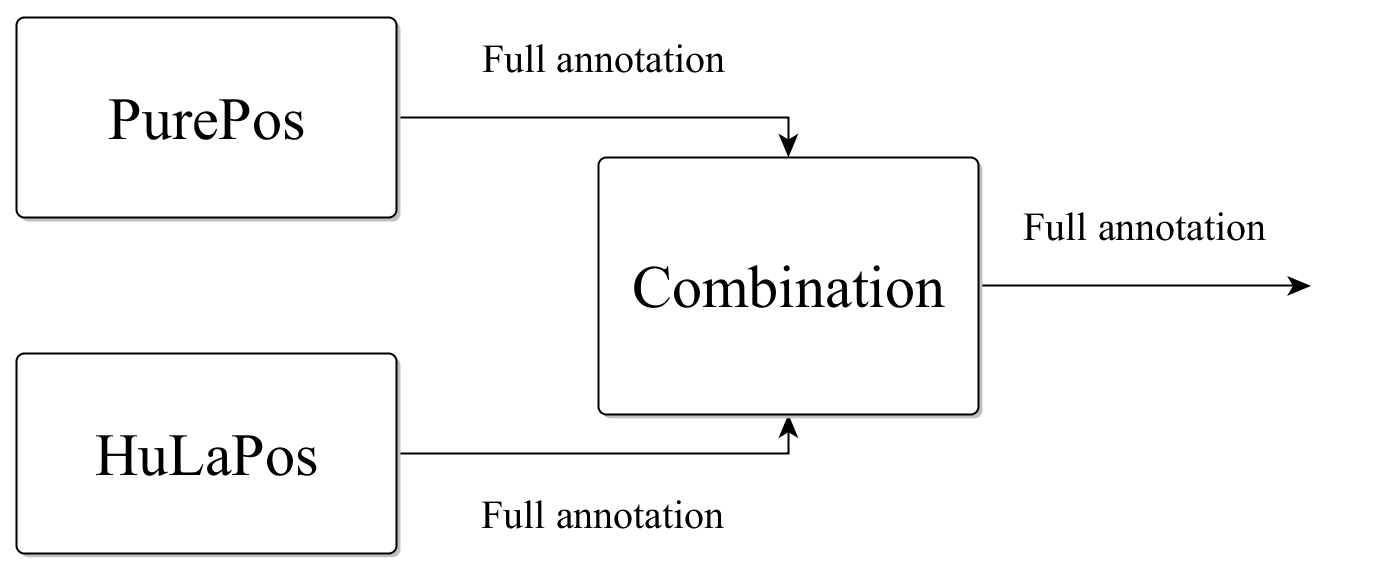
\includegraphics[scale=0.2]{MorphTagging/comb1.png} 
  \caption{Combining the output of two morphological taggers}
  \label{fig:comb1}
\end{figure}

\subsubsection{Combining PoS taggers only}

Another plausible scheme is to combine only the \acrshort{pos} tagger modules of the tools (see Figure \ref{fig:comb2}).
However, in doing so, one has to deal with lemmatization as well.
A straightforward solution for this to employ the lemmatizer of the better annotator tool (PurePos).
Following this way, the best tag selection model could be constructed (cf.
Table \ref{tab:comb-reduction-rates}) using IB learning with FS4 features.

\begin{figure}[H]
  \centering
  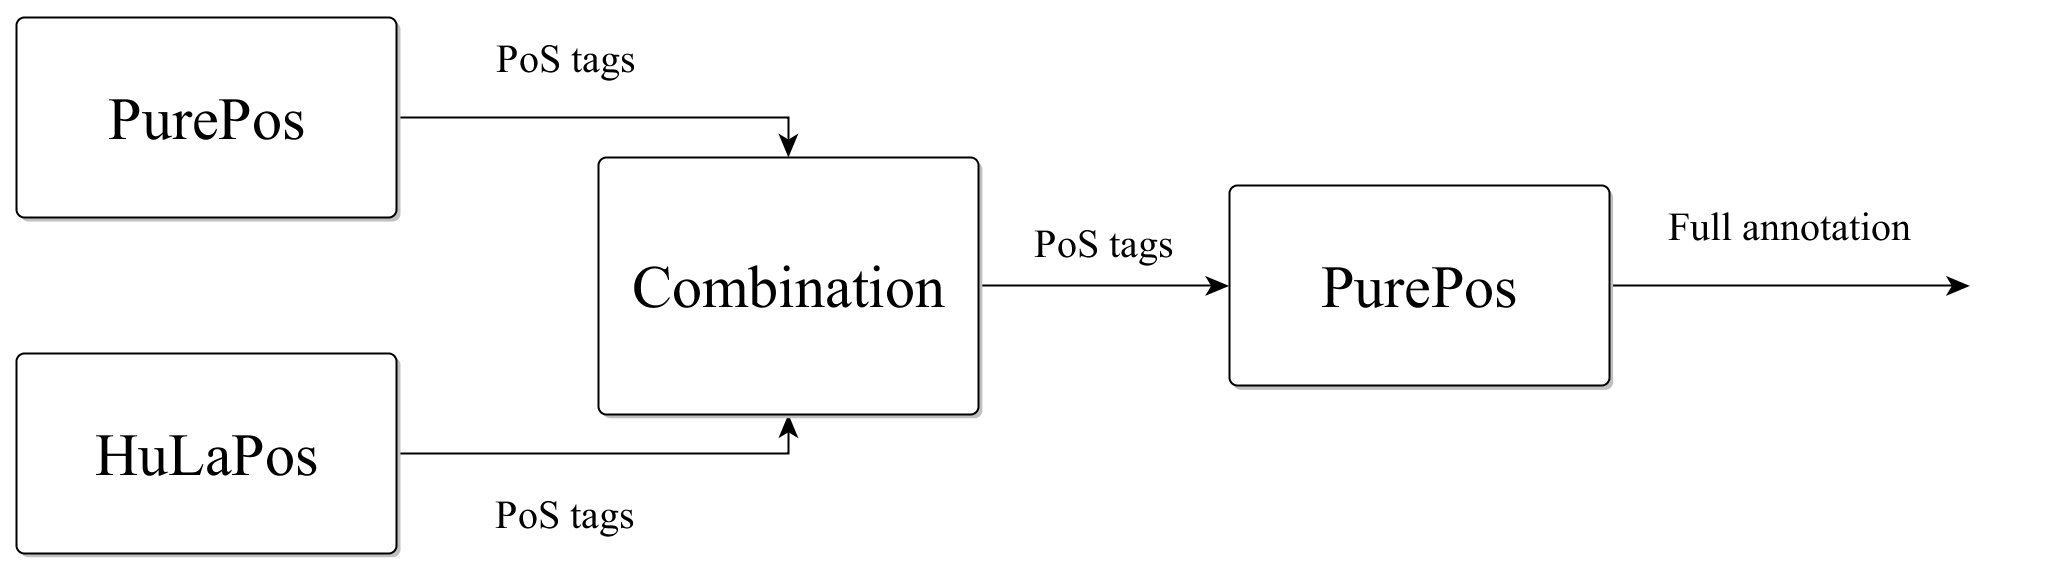
\includegraphics[scale=0.2]{MorphTagging/comb2.png} 
  \caption{Combining the output of two PoS taggers and using also a lemmatizer}
  \label{fig:comb2}
\end{figure}

Although this algorithm allows us to create a better morphosyntactic tagger compared to that of above, the gain in lemmatization remains much lower (6.81\%).
Consequently, the overall accuracy improvement measured in the development set (25.26\%) is inferior.

\subsubsection{Multiple metalearners}

Finally, the best results are produced using two level-1 learners: one of them chooses the better lemmatizer while the other selects the optimal \acrshort{pos} tagger (cf. Figure \ref{fig:comb3}).
In that  way, this architecture can incorporate the best lemma and tag candidates (as in Table \ref{tab:comb-reduction-rates}) yielding superior performance.
However, a drawback of this configuration that it may result in incompatible tag-lemma pairs\footnote{A lemma and a tag for a word is incompatible if the \acrshort{ma} can analyze the word, but no analysis contains both the lemma and the morphosyntactic label.}.
To overcome this problem, this combination scheme is enhanced with the Humor morphological analyzer.
This component is used to discover and fix incompatibilities.
With this enhancement, we achieved  32.42\% of improvement on the development set.

\begin{figure}[H]
  \centering
  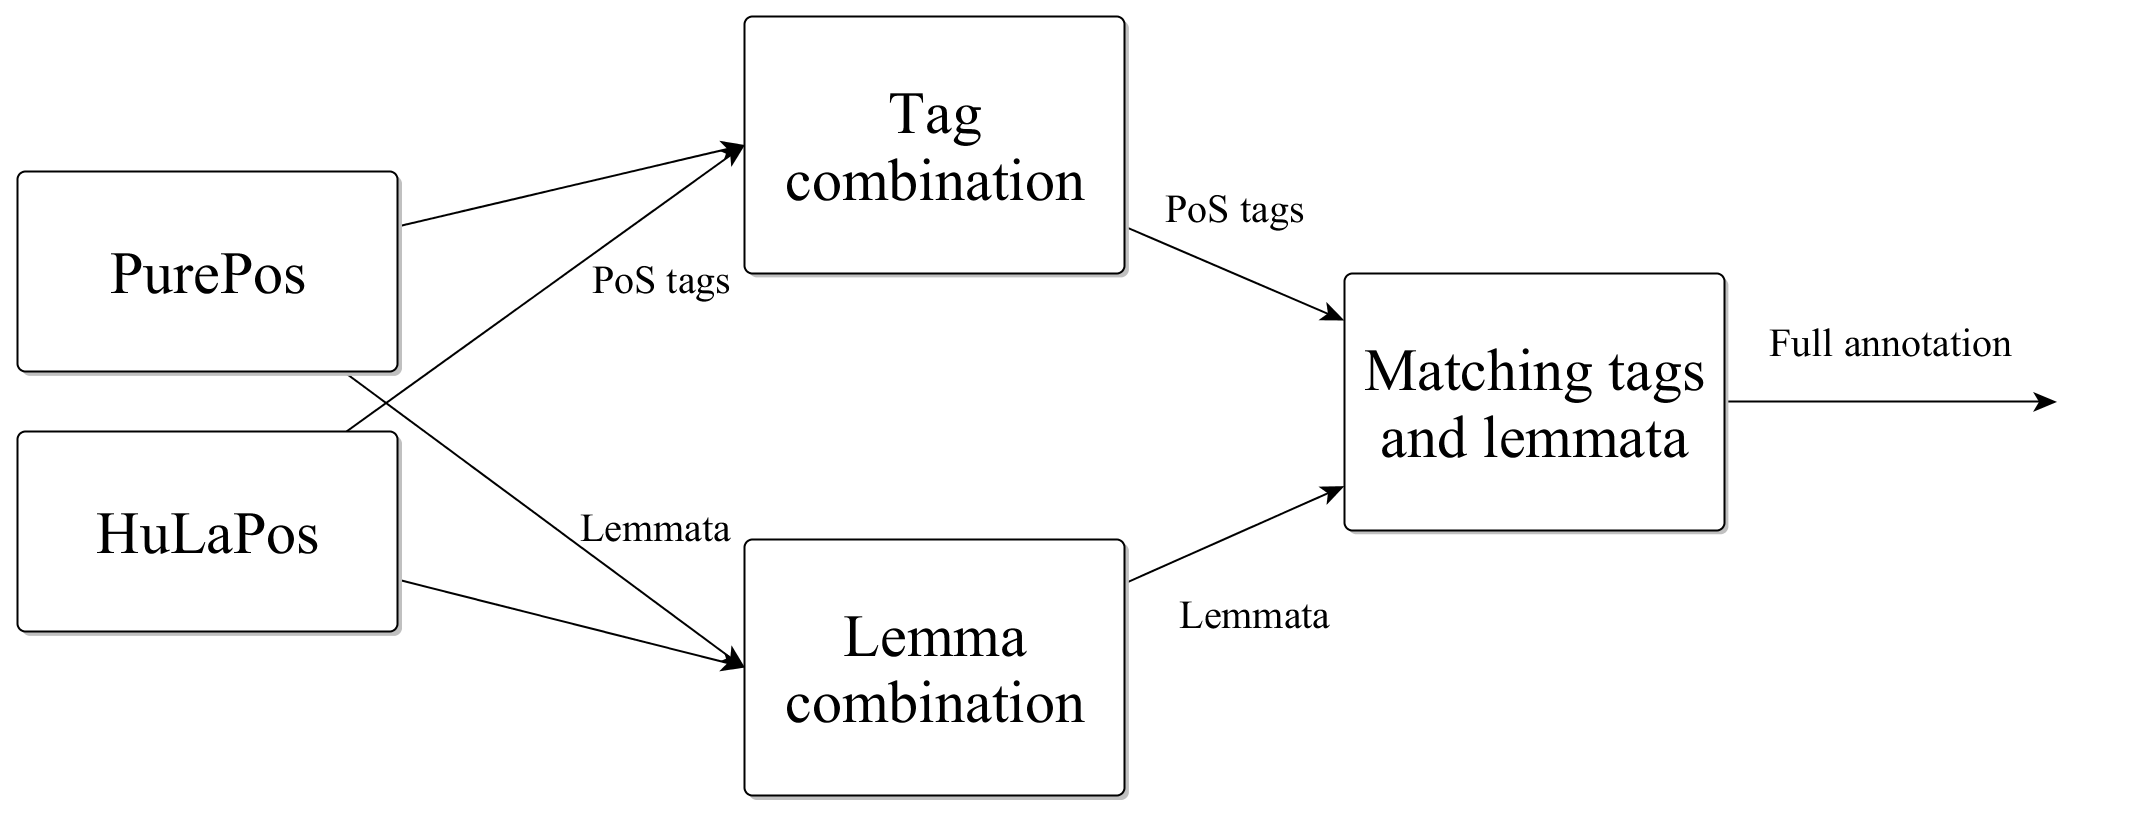
\includegraphics[scale=0.2]{MorphTagging/comb3.png} 
  \caption{Combining the output of two PoS taggers and lemmatizers}
  \label{fig:comb3}
\end{figure}

\subsection{Evaluation}

%In order to validate our hypothesis, stating that the last configuration performs the best, improvements
Combination schemes presented are evaluated on the unseen test set, confirming the results presented above.

\begin{table}[H]
\centering
\caption{Relative error rate reduction on the test set compared to PurePos}\label{tab:comb-eval}
\begin{tabular}{l r r r}
\hline
System & Tagging & Lemmatization & Full disamb. \\
\hline
Oracle & 48.60\% & 59.42\% & 51.53\% \\
Disamb. combination & 23.23\% & 23.55\% & 26.86\% \\
Tagger combination & 22.76\% & 13.77\% & 23.81\% \\
Multiple metalearners & 25.07\% & 29.89\% & \underline{28.90\%} \\
\hline
\end{tabular}
\end{table}

Results show (cf. Table \ref{tab:comb-eval}) that the hybrid architecture using a morphological analyzer achieved the best performance.
While other schemes could also increase the accuracy of PurePos, it resulted in the best tagging precision (98.90\%) of fixing 28.90\% of the baseline system's errors.
Further on, the proposed method also gives the highest error rate reduction in both \acrshort{pos} tagging and lemmatization.
These results show that our new combination architecture can be used in cases when very high disambiguation accuracy is crucial.
Finally, we also confirmed that PurePos and HuLaPos complement each other well resulting in an improved morphological tagger. 



 

 

 

 
